\documentclass[conference]{IEEEtran}
\usepackage[T1]{fontenc}
\usepackage{cite}
\usepackage{amsmath,amssymb}
\usepackage{graphicx}
\usepackage{booktabs}
\usepackage{array}
\usepackage{url}
\usepackage[hidelinks]{hyperref}
\graphicspath{{figures/}}
\begin{document}

\title{ViKAG-Faith: Graph-Grounded Claim-Level Faithfulness Evaluation and Verification for Vietnamese Knowledge-Augmented Generation}

\author{\IEEEauthorblockN{H\`a V\u{a}n Vinh}
\IEEEauthorblockA{Graduate student, Advanced Natural Language Processing\\
Vietnam}}

\maketitle

\begin{abstract}
Vietnamese RAG and GraphRAG question answering systems are usually scored with F1 or a single LLM-judge score for the whole answer. Neither shows which statements are backed by evidence and which are invented or contradicted. For legal regulations, one wrong effective date or fine is enough to cause harm. We build ViKAG-Faith, a claim-level faithfulness evaluation pipeline on ViHERMES. Two systems, Naive RAG and GraphRAG, answer 100 questions of 1--5 hops with Qwen2.5-3B. Answers are split into 610 claims, of which 284 claims from 80 answers are labelled supported, contradicted or unsupported against a common evidence set. We compare RAGAS, LLM-judges, SelfCheckGPT, multilingual NLI verifiers with and without graph information, number and date rules, verifiers fine-tuned on synthetic in-domain data, and a verify-then-revise loop. The primary labels are silver labels assigned by an LLM (Claude); 165 claims were also labelled blindly by one human annotator. On those claims, the 7B judge reaches the highest macro-F1 (0.528), above every NLI verifier (best 0.463). Fine-tuning with synthetic data raises the mDeBERTa verifier from 0.404 to 0.521 on silver labels, yet the gain disappears on human labels (0.381 versus 0.409). Silver labels agree with the human on 65\% of claims ($\kappa=0.29$), and metric rankings change with the label source. Verify-then-revise halves the contradiction rate but lowers token F1, because the small generator mostly deletes flagged claims.
\end{abstract}

\begin{IEEEkeywords}
GraphRAG, faithfulness, claim-level verification, Vietnamese, ViHERMES, meta-evaluation
\end{IEEEkeywords}

\section{Introduction}
GraphRAG and knowledge-augmented generation (KAG) bring knowledge graphs into retrieval to answer multi-step questions \cite{kag,graphrag,lightrag,hipporag}. ViHERMES \cite{vihermes} provides a multi-hop benchmark for Vietnamese healthcare regulations together with a legal structure graph, and shows that removing its Auditor (verification) module lowers the LLM-judge score from 0.7554 to 0.6823. Verification clearly matters, but the way faithfulness itself is measured on Vietnamese has not been evaluated.

An F1 or a single judge score for a whole answer does not reveal which statement is wrong. Common faithfulness metrics such as RAGAS \cite{ragas}, LLM-as-a-judge \cite{judge} and SelfCheckGPT \cite{selfcheck} have been validated mainly on English. DSC2025 ViHallu \cite{vihallu} evaluates Vietnamese hallucination, but not in connection with a knowledge graph or retrieved evidence.

Our approach splits answers into atomic claims, as FActScore \cite{factscore} does, checks each claim against a common evidence set of retrieved passages, gold passages and graph information, and measures how well each automatic metric matches reference labels. This is a meta-evaluation: the object under test is the checker, not the chatbot. We ask three questions.

\begin{itemize}
\item \textbf{RQ1:} How well do existing faithfulness metrics (RAGAS, LLM-judge, SelfCheckGPT, zero-shot NLI) match reference labels on Vietnamese?
\item \textbf{RQ2:} Do graph information, number and date rules, and fine-tuning on synthetic in-domain data help a verifier detect wrong claims better than a generic NLI verifier?
\item \textbf{RQ3:} How much does a verify-then-revise loop reduce unsupported claims, and does it hurt answer quality?
\end{itemize}

Our contributions are: (C1) a reproducible claim-level evaluation pipeline on ViHERMES; (C2) the pilot ViFaithKAG dataset with 284 silver-labelled claims, 165 human-labelled claims and the scores of every metric; (C3) a meta-evaluation of 24 metric variants, 12 in each of two rounds, with ablations of graph input, rules, synthetic data and revision rounds; and (C4) an analysis of LLM label reliability against a human annotator, showing that metric rankings depend on the label source.

\section{Related Work}
\textbf{Measuring RAG faithfulness.} RAGAS \cite{ragas} defines faithfulness as the share of statements that can be inferred from the context, using an LLM to extract and judge statements. FActScore \cite{factscore} scores each atomic fact against a knowledge source. LLM-as-a-judge \cite{judge} uses a strong LLM as the grader; agreement with humans depends on model size and domain.

\textbf{Hallucination detection.} SelfCheckGPT \cite{selfcheck} needs no evidence and relies on consistency between sampled answers. SemEval-2024 SHROOM \cite{shroom} and SemEval-2025 Mu-SHROOM \cite{mushroom} standardise the detection of invented spans, and DSC2025 ViHallu \cite{vihallu} is a Vietnamese challenge on this topic.

\textbf{Vietnamese and multilingual NLI.} XNLI \cite{xnli} includes Vietnamese, and ViNLI \cite{vinli} is a Vietnamese NLI corpus that is part of VLUE \cite{vlue}. mDeBERTa-v3 \cite{deberta}, trained on multilingual NLI \cite{mdeberta}, is a widely used encoder verifier.

\textbf{Graph RAG, KAG and regulations.} RAG \cite{rag}, GraphRAG \cite{graphrag}, LightRAG \cite{lightrag}, HippoRAG 2 \cite{hipporag} and KAG \cite{kag} use graphs for retrieval or reasoning. ViHERMES \cite{vihermes} builds a Document--Article--Clause graph with amendment, replacement and citation relations for healthcare documents.

\textbf{Positioning.} We do not propose a new QA system. We evaluate verification metrics on Vietnamese at claim level against human labels, keeping the ViHERMES data and graph unchanged and adding only an evaluation layer.

\section{Proposed Method}
Fig.~\ref{fig:pipeline} summarises the pipeline. The upper row generates answers with two systems, the lower row evaluates each claim, and the revise branch uses verification results to rewrite answers.

\begin{figure*}[t]
\centering
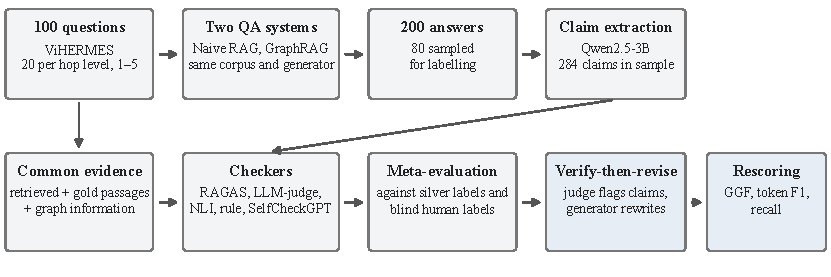
\includegraphics[width=\textwidth]{pipeline.pdf}
\caption{The ViKAG-Faith pipeline. Answers in the labelled sample go to claim extraction, then to the checkers and to meta-evaluation.}
\label{fig:pipeline}
\end{figure*}

\subsection{Question answering systems}
Both systems share the ViHERMES corpus (998 passages from 471 documents), a hybrid BM25 \cite{bm25} and bge-m3 \cite{bge} retriever (weight 0.5), a budget of 6,000 characters and the Qwen2.5-3B-Instruct generator \cite{qwen} at temperature 0. Naive RAG takes the 8 best passages. GraphRAG takes 4 seed passages, propagates over the ViHERMES graph (depth up to 4, at most 8 nodes) and adds a list of document relations to the prompt. Any difference between the systems therefore comes only from how context is obtained.

\subsection{Claim extraction and common evidence}
Qwen2.5-3B extracts claims with a Vietnamese prompt containing two examples. Each claim must have one main predicate and stand alone, with pronouns replaced by names and numbers, dates and document identifiers kept intact. For each answer, the evidence is the union of the retrieved passages and the gold passages of the question, with the graph information of each passage (document title, identifier and relations). Every metric and the annotator use exactly this set, so differences between metrics reflect metric quality and not retrieval quality.

\subsection{Labels and answer-level metrics}
Each claim receives one label from supported, contradicted and unsupported. For an answer with claim set $C$, the faithfulness score GGF is the share of supported claims, and CR and UR are the contradicted and unsupported rates:
\begin{equation}
\mathrm{GGF}=\frac{|\{c\in C: c\ \text{supported}\}|}{|C|},
\end{equation}
\begin{equation}
\mathrm{CR}=\frac{|\{c\in C: c\ \text{contradicted}\}|}{|C|},\quad
\mathrm{UR}=\frac{|\{c\in C: c\ \text{unsupported}\}|}{|C|}.
\end{equation}

\subsection{Checkers}
\textbf{LLM-based metrics.} RAGAS faithfulness is reimplemented from the two original prompts of the library, and a claim-level LLM-judge assigns the three labels to our claims. Both run with Qwen2.5-3B and 7B through Ollama; round 2 adds 14B and a Qwen 3B verifier that returns a label with an evidence span. Unreadable outputs are excluded from measurement and never defaulted to a label.

\textbf{NLI verifier.} mDeBERTa-v3-base-xnli-multilingual \cite{deberta,mdeberta} runs on windows of 900 characters with a stride of 700; round 2 adds XLM-R large xnli, zero-shot and fine-tuned on 16,000 pairs. For claim $c$ and windows $w$,
\begin{equation}
P_{\mathrm{sup}}(c)=\max_{w}\,P(\mathrm{entail}\mid w,c),
\end{equation}
\begin{equation}
P_{\mathrm{con}}(c)=\max_{w\in W_2(c)}\,P(\mathrm{contradiction}\mid w,c),
\end{equation}
where $W_2(c)$ holds the two windows with the highest word overlap with the claim, because NLI models tend to return contradiction for unrelated text. A claim is supported if $P_{\mathrm{sup}}\ge\tau_s$, otherwise contradicted if $P_{\mathrm{con}}\ge\tau_c$, and otherwise unsupported. The thresholds are chosen on the dev split (V1 zero-shot: $\tau_s=0.65$, $\tau_c=0.45$). V1 uses passages only. V2 adds the document title, identifier and relations to the start of every window. V3 adds at most 3 triples sharing keywords with the claim, from 467 graph triples, and, through a mutual index, the source passage of any document the claim cites.

\textbf{Fine-tuning on synthetic data.} We combine 12,000 ViNLI \cite{vinli} pairs with 3,328 pairs built from passages outside the evaluation sample: supported is the original sentence; contradicted changes a number or date or adds a negation; unsupported is a sentence from another passage of the same document. Training runs one epoch at learning rate $5\times10^{-6}$, batch size 4 with 4 accumulation steps, in float32, keeping the best dev checkpoint. An ablation uses ViNLI only. Round 2 repeats this with 12,000 ViNLI pairs and 17,993 synthetic pairs. A first run on a 4 GB GPU had to shorten training premises to 450 characters and 200 tokens; it was then repeated with the round 1 input of 900 characters and 320 tokens.

\textbf{Rules and SelfCheckGPT.} A number, date or identifier in a claim that is missing from the evidence demotes supported to unsupported; if the matching evidence sentence holds a different value of the same kind, the claim becomes contradicted. SelfCheckGPT-NLI \cite{selfcheck} samples 3 extra answers at temperature 0.7 from the same prompt and context, and averages the mDeBERTa entailment and contradiction probabilities using each sample as premise. It does not see the evidence.

\subsection{Verify-then-revise}
For RQ3, the 7B judge flags unsupported or contradicted claims. Qwen2.5-3B receives the same retrieved context, the old answer and the flagged claims, and rewrites the answer by fixing or dropping them. The new answer is split into claims and rescored by the 7B judge, for at most 2 rounds.

\section{Dataset}
We draw 100 of the 1,561 ViHERMES questions by stratified sampling (20 per hop level, seed 42), so two systems give 200 answers. The labelled sample has 40 questions (8 per hop level) for 80 answers and 284 claims (Table~\ref{tab:data}).

\begin{table}[t]
\caption{Dataset statistics}
\label{tab:data}
\centering
\footnotesize
\begin{tabular}{p{0.46\columnwidth}p{0.44\columnwidth}}
\toprule
Item & Value \\
\midrule
Questions / hop levels & 100 / 20 per level, 1--5 \\
Answers (two systems) & 200 \\
Labelled sample & 80 answers, 284 claims (15 malformed claims excluded) \\
Silver label distribution & supported 184, contradicted 42, unsupported 43 \\
Dev / test split by question & 51 / 218 claims \\
\bottomrule
\end{tabular}
\end{table}

Synthetic pairs come from passages outside the evaluation sample, so they do not leak into the test split. The dev set holds 1,000 ViNLI pairs and 10\% of the synthetic pairs. Table~\ref{tab:dev} shows that synthetic data strongly raises accuracy on synthetic pairs, while the ViNLI-only model barely learns the in-domain error types.

\begin{table}[t]
\caption{Verifier accuracy on the dev set (three labels)}
\label{tab:dev}
\centering
\footnotesize
\begin{tabular}{lcc}
\toprule
Verifier & ViNLI dev & Synthetic dev \\
\midrule
mDeBERTa zero-shot & 0.758 & 0.545 \\
Fine-tuned, ViNLI + synthetic & 0.793 & 0.875 \\
Fine-tuned, ViNLI only & 0.798 & 0.588 \\
\bottomrule
\end{tabular}
\end{table}

\textbf{Silver labels.} Claude labelled all claims with evidence passage numbers and reasons. These labels are the reference for every test-set measurement, but they are not human labels.

\textbf{Human labels (blind audit).} One annotator worked on an offline HTML page without seeing Claude's labels or reasons, and without knowing which system produced an answer. Pass C covers 60 claims stratified by Claude's label (30/15/15) with full passages. Passes G, H, I and J each cover 30 random claims not used before, one claim per screen with the 4 most overlapping evidence sentences and the option to open the full passage. A pre-filled review pass (A) and two passes with exports not created through the labelling page (D, E) were excluded (Table~\ref{tab:audit}).

\begin{table}[t]
\caption{Human labelling passes}
\label{tab:audit}
\centering
\footnotesize
\begin{tabular}{p{0.2\columnwidth}p{0.3\columnwidth}ccc}
\toprule
Pass & Selection and display & Claims & Agree & $\kappa$ \\
\midrule
C & Stratified, full passage & 60 & 60\% & 0.29 \\
G, H, I, J & Random, 4 sentences & 105 & 69\% & 0.30 \\
All & & 165 & 65\% & 0.29 \\
Excluded & A, D, E & -- & -- & -- \\
\bottomrule
\end{tabular}
\end{table}

Table~\ref{tab:examples} shows three claims where the human label equals Claude's label, translated from Vietnamese.

\begin{table}[t]
\caption{Example claims and evidence (translated)}
\label{tab:examples}
\centering
\footnotesize
\begin{tabular}{p{0.36\columnwidth}p{0.36\columnwidth}p{0.16\columnwidth}}
\toprule
Claim & Evidence & Label \\
\midrule
The total fine of the three clinics is 8 million VND. & One clinic alone was fined 30,000,000 VND. & contra. \\
The Population Department has no role in inspection or handling violations. & Its duties include specialised inspection and handling violations in the population field. & contra. \\
Circular 30/2017/TT-BYT takes effect on 01/01/2018. & The evidence gives no such date. & unsup. \\
\bottomrule
\end{tabular}
\end{table}

\section{Experimental Setup}
\textbf{Configurations.} Round 1 compares 12 variants: LLM-judge and RAGAS with 3B and 7B; NLI zero-shot, fine-tuned and ViNLI-only, each with V1 and V2; SelfCheckGPT-NLI; and rule only. Each NLI variant is also tested with and without rules, and an always-supported baseline is included. Round 2 adds 12 variants: judge and RAGAS 14B, zero-shot V3, fine-tuned V1 and V3 at 450 and 900 characters, XLM-R zero-shot and fine-tuned V1 and V3, and Qwen 3B with spans.

\textbf{Metrics.} At claim level we report three-label macro-F1, per-label F1 and AUROC for detecting non-supported claims. At answer level we report Spearman and Kendall correlation between automatic scores and reference GGF on 61--63 test answers, depending on valid outputs. For revision we report changes in GGF, CR, UR, token F1, exact match and token recall against ViHERMES answers.

\textbf{Statistics.} We use 95\% bootstrap confidence intervals with 1,000 resamples, paired bootstrap for macro-F1 differences, paired Wilcoxon tests for system and before/after comparisons, and Cohen's $\kappa$ for agreement. Intervals are not corrected for multiple comparisons.

\textbf{Hardware.} Models run on a Google Colab T4 GPU (Ollama with Q4\_K\_M quantisation; PyTorch in float32), except zero-shot V3 on CPU and the short-premise fine-tune on a local GTX 1650.

\section{Results}
Table~\ref{tab:main} and Fig.~\ref{fig:scores} give the main results of round 1.

\begin{table*}[t]
\caption{Main results of round 1. Macro-F1, CI and AUROC on 218 test claims (silver labels); human column on 165 human-labelled claims; Spearman $\rho$ between answer scores and reference GGF}
\label{tab:main}
\centering
\footnotesize
\begin{tabular}{lccccc}
\toprule
Method & Macro-F1 & 95\% CI & AUROC & Macro-F1 (human) & Spearman $\rho$ \\
\midrule
LLM-judge Qwen2.5-7B & 0.476 & [0.40, 0.55] & 0.748 & 0.528 & 0.418 \\
LLM-judge Qwen2.5-3B & 0.439 & [0.37, 0.53] & 0.643 & 0.349 & 0.367 \\
NLI fine-tuned, V1 & 0.521 & [0.44, 0.60] & 0.738 & 0.381 & 0.142 \\
NLI fine-tuned, V2 (+graph) & 0.465 & [0.39, 0.54] & 0.735 & 0.336 & 0.383 \\
NLI fine-tuned ViNLI only, V1 & 0.405 & [0.33, 0.47] & 0.649 & 0.395 & $-$0.005 \\
NLI zero-shot, V1 & 0.404 & [0.33, 0.47] & 0.545 & 0.409 & 0.003 \\
NLI zero-shot V1 + rule & 0.401 & [0.33, 0.47] & 0.534 & 0.413 & 0.012 \\
NLI zero-shot, V2 (+graph) & 0.329 & [0.27, 0.39] & 0.534 & 0.295 & 0.161 \\
SelfCheckGPT-NLI & 0.409 & [0.34, 0.48] & 0.600 & 0.336 & 0.270 \\
Rule only & 0.274 & [0.26, 0.29] & 0.513 & 0.310 & 0.147 \\
Always supported & 0.275 & [0.26, 0.29] & 0.500 & 0.279 & -- \\
RAGAS (Qwen2.5-7B) & -- & -- & -- & -- & 0.484 \\
RAGAS (Qwen2.5-3B) & -- & -- & -- & -- & 0.258 \\
\bottomrule
\end{tabular}
\end{table*}

\begin{figure}[t]
\centering
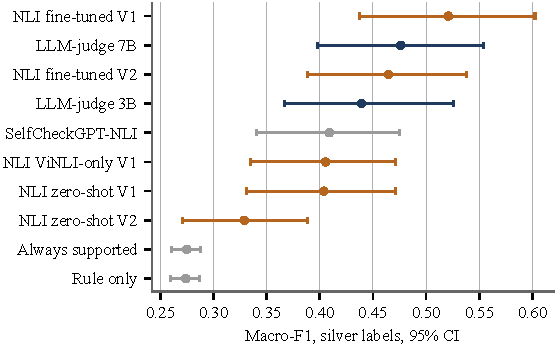
\includegraphics[width=\columnwidth]{scores.pdf}
\caption{Claim-level macro-F1 on the test split. Blue: LLM-judges; orange: NLI verifiers; grey: SelfCheckGPT, rule and baseline.}
\label{fig:scores}
\end{figure}

\subsection{RQ1: Existing metrics}
In round 1, among methods that need no training, the 7B judge is best at claim level (macro-F1 0.476, AUROC 0.748), ahead of the 3B judge (0.439) and zero-shot NLI (0.404). It catches 41/64 wrong claims and raises 22/153 false alarms. All methods are weak on the two error labels (Table~\ref{tab:class}). SelfCheckGPT-NLI reaches 0.409, level with zero-shot NLI without seeing the evidence, but its accuracy is low (0.463) because it treats correct claims as doubtful when samples are worded differently. At answer level, RAGAS 7B has the highest correlation with reference GGF ($\rho=0.484$) while RAGAS 3B reaches only 0.258, so judge size matters more than the metric formula. High accuracy does not imply a good metric: always predicting supported gives accuracy 0.702, which is why macro-F1 is our main measure.

\begin{table}[t]
\caption{F1 per label on the test split (silver labels)}
\label{tab:class}
\centering
\footnotesize
\begin{tabular}{lcccc}
\toprule
Method & Supp. & Contra. & Unsup. & Acc. \\
\midrule
Judge 7B & 0.853 & 0.321 & 0.254 & 0.687 \\
Judge 3B & 0.825 & 0.129 & 0.364 & 0.692 \\
Fine-tuned V1 & 0.773 & 0.379 & 0.410 & 0.656 \\
Zero-shot V1 & 0.737 & 0.308 & 0.167 & 0.592 \\
SelfCheckGPT & 0.565 & 0.400 & 0.262 & 0.463 \\
Rule only & 0.822 & 0.000 & 0.000 & 0.688 \\
\bottomrule
\end{tabular}
\end{table}

\subsection{RQ2: Graph, rules and fine-tuning}
Adding graph information to every window (V2) lowers zero-shot macro-F1 from 0.404 to 0.329. Its best threshold is very low ($\tau_s=0.15$): with a document title at the start of each window, the model gives high entailment to any claim naming that document. Adding only triples related to each claim (V3) raises zero-shot macro-F1 to 0.423, above V2, but on human labels V3 falls below V1 (0.328 versus 0.409). Rules barely change results (0.404 to 0.401), since many errors concern the wrong subject and not a number. On silver labels, fine-tuned V1 beats zero-shot (difference 0.117, 95\% CI [0.03, 0.20]) and is not significantly above the 7B judge. The ViNLI-only ablation shows no gain (0.002), so the improvement comes from the synthetic in-domain data (Table~\ref{tab:paired}).

\begin{table}[t]
\caption{Paired comparison of macro-F1 on the test split (silver labels, 1,000 bootstrap resamples)}
\label{tab:paired}
\centering
\footnotesize
\begin{tabular}{p{0.46\columnwidth}ccc}
\toprule
Comparison & Diff. & 95\% CI & Share $\le 0$ \\
\midrule
Fine-tuned V1 $-$ judge 7B & 0.047 & [$-$0.06, 0.16] & 0.188 \\
Fine-tuned V1 $-$ zero-shot V1 & 0.117 & [0.03, 0.20] & 0.006 \\
Fine-tuned V1 $-$ ViNLI only & 0.115 & [0.05, 0.18] & 0.000 \\
ViNLI only $-$ zero-shot V1 & 0.002 & [$-$0.06, 0.06] & 0.475 \\
Fine-tuned V1 $-$ fine-tuned V2 & 0.056 & [$-$0.01, 0.12] & 0.056 \\
Judge 7B $-$ SelfCheckGPT & 0.065 & [$-$0.05, 0.17] & 0.120 \\
\bottomrule
\end{tabular}
\end{table}

\textbf{Human labels.} Fig.~\ref{fig:labels} reverses the conclusion on fine-tuning. On 165 claims, fine-tuned V1 reaches 0.381, level with zero-shot (0.409) and clearly below the 7B judge (0.528). The rank correlation of metrics between the two label sets is only $\rho=0.46$. Verifier thresholds are chosen on Claude's labels, so the fine-tuned model may have learnt Claude's strict labelling. Table~\ref{tab:confusion} supports this: Claude labels 59 claims contradicted or unsupported, and the human agrees on only 18 and labels 29 of them supported, whereas 85\% of Claude's supported labels are confirmed.

\begin{figure}[t]
\centering
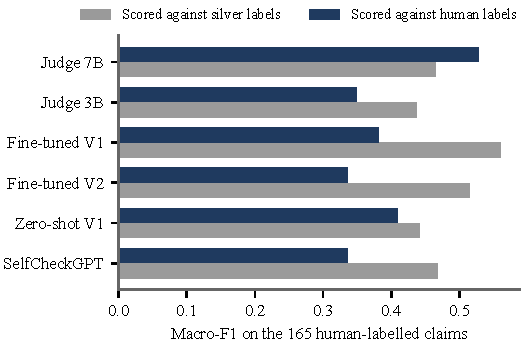
\includegraphics[width=\columnwidth]{labels.pdf}
\caption{Macro-F1 of metrics on the human-labelled claims, scored against each label set.}
\label{fig:labels}
\end{figure}

\begin{table}[t]
\caption{Confusion between Claude labels (rows) and human labels (columns) on 165 claims}
\label{tab:confusion}
\centering
\footnotesize
\begin{tabular}{lcccc}
\toprule
Claude & Supp. & Contra. & Unsup. & Agree \\
\midrule
supported & 90 & 5 & 11 & 85\% \\
contradicted & 16 & 8 & 6 & 27\% \\
unsupported & 13 & 6 & 10 & 34\% \\
\bottomrule
\end{tabular}
\end{table}

\textbf{Round 2: larger models.} The 14B judge reaches 0.541 on silver labels, not significantly different from the 7B judge (0.069, CI [$-$0.05, 0.18]). On human labels it is lower (0.439 versus 0.528, CI of the difference [$-$0.20, 0.03]). At answer level, RAGAS 14B reaches $\rho=0.644$ and the 14B judge 0.597, above the 7B versions (0.484 and 0.418), but on 61 answers and without a test of the difference. XLM-R zero-shot V1 reaches 0.532 on silver labels, clearly above mDeBERTa zero-shot (0.128, CI [0.03, 0.22]), but only 0.354 on human labels. XLM-R fine-tuned V1 reaches 0.463 on human labels, significantly above XLM-R zero-shot (0.109, CI [0.02, 0.20]) and not significantly different from the 7B judge (CI [$-$0.17, 0.04]), at the cost of 64/153 false alarms. XLM-R fine-tuned V3 has the highest AUROC (0.821), above round 1 on silver labels (CI [0.01, 0.16]) but not on human labels. Qwen 3B with spans reaches 0.361 on silver and 0.399 on human labels, clearly below the 7B judge; only 130/263 labels carry a span copied from the evidence, ignoring case and punctuation.

\textbf{Round 2: about 20,000 synthetic pairs.} Accuracy on synthetic dev pairs rises from 0.594 to 0.897. With short premises (450 characters, 200 tokens), fine-tuned V1 reaches only 0.441, below round 1 ($-$0.080, CI [$-$0.16, 0.00]). Retraining with the round 1 input (900 characters, 320 tokens) gives 0.572, the highest silver score, significantly above the short-premise model (0.131, CI [0.05, 0.22]) but not above round 1 (0.051, CI [$-$0.02, 0.12]). AUROC barely moves (0.738 to 0.754, CI [$-$0.01, 0.04]). The first drop thus came from short premises, and more data did not improve discrimination. On human labels this model reaches only 0.356, clearly below the 7B judge (CI [$-$0.28, $-$0.05]). Table~\ref{tab:round2} lists these results.

\begin{table*}[t]
\caption{Round 2 on the test split compared with round 1 and the 7B judge. Thresholds are chosen on dev with the round 1 grid. ``Caught'' counts wrong claims detected; ``False alarms'' counts correct claims flagged}
\label{tab:round2}
\centering
\footnotesize
\begin{tabular}{lcccccc}
\toprule
Method & Silver & 95\% CI & AUROC & Caught & False alarms & Human \\
\midrule
Judge 7B & 0.476 & [0.40, 0.55] & 0.748 & 41/64 & 22/153 & 0.528 \\
Judge 14B & 0.541 & [0.46, 0.62] & 0.761 & 45/65 & 26/153 & 0.439 \\
Fine-tuned V1, round 1 & 0.521 & [0.44, 0.60] & 0.738 & 34/65 & 37/153 & 0.381 \\
Fine-tuned V1, 450 chars & 0.441 & [0.36, 0.53] & 0.753 & 16/65 & 15/153 & 0.371 \\
Fine-tuned V1, 900 chars & 0.572 & [0.48, 0.64] & 0.754 & 44/65 & 48/153 & 0.356 \\
Fine-tuned V3, 900 chars & 0.559 & [0.48, 0.63] & 0.734 & 50/65 & 57/153 & 0.346 \\
XLM-R zero-shot V1 & 0.532 & [0.45, 0.61] & 0.743 & 33/65 & 36/153 & 0.354 \\
XLM-R fine-tuned V1 & 0.500 & [0.42, 0.57] & 0.798 & 58/65 & 64/153 & 0.463 \\
XLM-R fine-tuned V3 & 0.477 & [0.40, 0.55] & 0.821 & 60/65 & 62/153 & 0.433 \\
Qwen 3B with spans & 0.361 & [0.30, 0.43] & 0.601 & 23/65 & 23/151 & 0.399 \\
\bottomrule
\end{tabular}
\end{table*}

\subsection{RQ3: Verify-then-revise}
Of 80 answers, 42 have flagged claims (Table~\ref{tab:revise}). GGF rises from 0.755 to 0.830 (Wilcoxon $p=0.014$) and CR halves, but token F1 falls from 0.595 to 0.563 ($p=0.001$), claims per answer fall from 3.55 to 2.44, and 7 answers become ``no information found''. Round 1 of revision gives most of the gain. Exact match is 0 in every configuration because ViHERMES answers are long (about 115 words), so token recall measures content loss. The GGF gain is an upper bound, since the 7B judge both flags and rescores.

\begin{table}[t]
\caption{Verify-then-revise on 80 answers. GGF, CR and UR from the 7B judge; F1, recall and EM against ViHERMES answers}
\label{tab:revise}
\centering
\footnotesize
\setlength{\tabcolsep}{3pt}
\begin{tabular}{lccccccc}
\toprule
Setting & GGF & CR & UR & F1 & Recall & EM & Claims \\
\midrule
No revision & 0.755 & 0.088 & 0.157 & 0.595 & 0.591 & 0.000 & 3.55 \\
At most 1 round & 0.801 & 0.059 & 0.140 & 0.569 & 0.545 & 0.000 & 2.75 \\
At most 2 rounds & 0.830 & 0.041 & 0.129 & 0.563 & 0.535 & 0.000 & 2.44 \\
\bottomrule
\end{tabular}
\end{table}

In one 3-hop example, the 7B judge flagged the claim that the amended Pharmacy Law would go to the National Assembly in 10/2025, while the document says 10/2022. The new answer reached GGF of 1 by the judge but dropped all three dates, including the correct 01/07/2025 date that both the judge and Claude labelled supported, and replaced them with a generic sentence saying the dates are stated in the context. This pattern explains how GGF rises while token recall falls.

\subsection{Systems and hop difficulty}
The two systems do not differ significantly (paired Wilcoxon on GGF, $p=0.191$; Table~\ref{tab:systems}). The released ViHERMES graph is coarse, with few amendment edges, so propagation adds few gold passages. Faithfulness falls clearly at 4 and 5 hops (Fig.~\ref{fig:hops}).

\begin{table}[t]
\caption{Answer quality and faithfulness of the two systems}
\label{tab:systems}
\centering
\footnotesize
\begin{tabular}{lccccc}
\toprule
System & Token F1 & Gold recall & GGF & CR & UR \\
\midrule
Naive RAG & 0.570 & 47.0\% & 0.694 & 0.182 & 0.124 \\
GraphRAG & 0.563 & 47.9\% & 0.638 & 0.199 & 0.163 \\
\bottomrule
\end{tabular}
\end{table}

\begin{figure}[t]
\centering
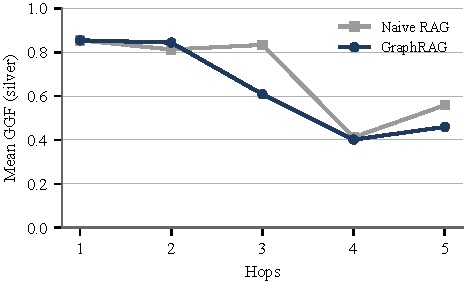
\includegraphics[width=\columnwidth]{hops.pdf}
\caption{Mean GGF by hop count, with 8 questions per level. GraphRAG has 7 answers with claims at 5 hops.}
\label{fig:hops}
\end{figure}

\subsection{Error analysis}
\begin{itemize}
\item \textbf{Wrong dates:} an answer places the amended Pharmacy Law in 10/2025, while the document says 10/2022; 10/2025 belongs to the Food Safety Law.
\item \textbf{Wrong subject:} a task of the Ministry Office is assigned to the Institute of Strategy and Policy. Number and date rules cannot catch this type.
\item \textbf{Wrong aggregation:} fines from several decisions are added incorrectly. Both LLM-judges miss this because they must add numbers across documents; NLI catches it.
\item \textbf{Invented lists:} an answer lists Instagram, TikTok and YouTube although the advertising certificate names others; zero-shot NLI is misled because another document in the context mentions Instagram.
\item \textbf{False refusals and extraction errors:} answers claim there is no information when the evidence is explicit, and 15 claims were malformed by extraction.
\end{itemize}

\section{Threats to Validity}
\textbf{Silver reference.} Claude agrees with the human on 65\% of claims ($\kappa=0.29$). We therefore report both label sets; more human labels and a second annotator with adjudication are needed.

\textbf{One annotator.} The annotator is not a legal expert, and quick passes show 4 evidence sentences, so distant evidence may be missed. Pass C uses full passages and is reported separately.

\textbf{Small scale.} We evaluate 2 systems, 284 claims and judges up to 14B. Bootstrap intervals and paired tests accompany the main comparisons, without multiple-comparison correction.

\textbf{Thresholds tuned on silver labels.} This biases fine-tuned verifiers toward Claude, and only 51 dev claims are available. Thresholds should be selected on human labels when enough exist.

\textbf{Self-scored revision.} Revised answers are scored only by the judge that flagged them. Rescoring by humans or an independent metric is needed.

\textbf{Graph as text.} Triples are appended as text, so verifiers do not read graph structure. ViEduReg and the KAG Verify operator are not covered.

\section{Conclusion}
On Vietnamese healthcare regulations, automatic faithfulness metrics running on small open LLMs match reference labels only at a low to moderate level. The 7B judge is the most stable metric across both label sets, and the 14B judge is not significantly better at claim level. RAGAS is best at answer level and improves with model size. Fine-tuning mDeBERTa on synthetic in-domain data raises silver scores but not human-label scores, and about 20,000 pairs bring no significant gain; XLM-R fine-tuning improves on human labels but raises many false alarms. Meta-evaluation with LLM labels can therefore change metric rankings. Verify-then-revise with a 3B generator reduces wrong claims by deleting content, which is a trade-off and not a pure improvement.

Future work includes full human labelling by two annotators with legal expertise and threshold selection on human labels; a 32B judge and a fine-tuned small Qwen verifier whose spans are copied from the evidence; structured triple input for verifiers and extension to LightRAG, HippoRAG 2, KAG and ViEduReg; and independent scoring of revised answers with a larger generator. Code and data are available at \url{https://github.com/vinhha195-oss/vikag-faith}.

\begin{thebibliography}{99}
\bibitem{kag} L. Liang \emph{et al.}, ``KAG: Boosting LLMs in professional domains via knowledge augmented generation,'' 2024, arXiv:2409.13731.
\bibitem{graphrag} D. Edge, H. Trinh, N. Cheng \emph{et al.}, ``From local to global: A graph RAG approach to query-focused summarization,'' 2024, arXiv:2404.16130.
\bibitem{lightrag} Z. Guo, L. Xia, Y. Yu, T. Ao, and C. Huang, ``LightRAG: Simple and fast retrieval-augmented generation,'' 2024, arXiv:2410.05779.
\bibitem{hipporag} B. J. Guti\'errez, Y. Shu, W. Qi, S. Zhou, and Y. Su, ``From RAG to memory: Non-parametric continual learning for large language models,'' 2025, arXiv:2502.14802.
\bibitem{vihermes} L. S. T. Nguyen, Q. M. Bui, T. T. Ngo, Q. T. N. Vo, D. N. H. Le, and T. T. Quan, ``ViHERMES: A graph-grounded multihop question answering benchmark and system for Vietnamese healthcare regulations,'' in \emph{Proc. ACIIDS}, 2026, arXiv:2602.07361.
\bibitem{ragas} S. Es, J. James, L. Espinosa-Anke, and S. Schockaert, ``RAGAs: Automated evaluation of retrieval augmented generation,'' in \emph{Proc. EACL System Demonstrations}, 2024.
\bibitem{judge} L. Zheng, W.-L. Chiang, Y. Sheng \emph{et al.}, ``Judging LLM-as-a-judge with MT-Bench and Chatbot Arena,'' in \emph{Proc. NeurIPS}, vol. 36, 2023, arXiv:2306.05685.
\bibitem{selfcheck} P. Manakul, A. Liusie, and M. J. F. Gales, ``SelfCheckGPT: Zero-resource black-box hallucination detection for generative large language models,'' in \emph{Proc. EMNLP}, 2023, arXiv:2303.08896.
\bibitem{vihallu} ``DSC2025 ViHallu: Vietnamese hallucination detection challenge,'' 2026, arXiv:2601.04711.
\bibitem{factscore} S. Min, K. Krishna, X. Lyu \emph{et al.}, ``FActScore: Fine-grained atomic evaluation of factual precision in long form text generation,'' in \emph{Proc. EMNLP}, 2023, arXiv:2305.14251.
\bibitem{shroom} T. Mickus, E. Zosa, R. V\'azquez \emph{et al.}, ``SemEval-2024 Task 6: SHROOM, a shared-task on hallucinations and related observable overgeneration mistakes,'' in \emph{Proc. SemEval}, 2024, arXiv:2403.07726.
\bibitem{mushroom} R. V\'azquez, T. Mickus \emph{et al.}, ``SemEval-2025 Task 3: Mu-SHROOM, the multilingual shared task on hallucinations and related observable overgeneration mistakes,'' in \emph{Proc. SemEval}, 2025.
\bibitem{xnli} A. Conneau, R. Rinott, G. Lample \emph{et al.}, ``XNLI: Evaluating cross-lingual sentence representations,'' in \emph{Proc. EMNLP}, 2018.
\bibitem{vinli} T. V. Huynh, K. V. Nguyen, and N. L.-T. Nguyen, ``ViNLI: A Vietnamese corpus for studies on open-domain natural language inference,'' in \emph{Proc. COLING}, 2022.
\bibitem{vlue} ``VLUE: Vietnamese language understanding evaluation benchmark,'' 2024, arXiv:2403.15882.
\bibitem{deberta} P. He, J. Gao, and W. Chen, ``DeBERTaV3: Improving DeBERTa using ELECTRA-style pre-training with gradient-disentangled embedding sharing,'' in \emph{Proc. ICLR}, 2023, arXiv:2111.09543.
\bibitem{mdeberta} M. Laurer \emph{et al.}, ``mDeBERTa-v3-base-xnli-multilingual-nli-2mil7,'' Hugging Face model card. [Online]. Available: \url{https://huggingface.co/MoritzLaurer/mDeBERTa-v3-base-xnli-multilingual-nli-2mil7}
\bibitem{rag} P. Lewis, E. Perez, A. Piktus \emph{et al.}, ``Retrieval-augmented generation for knowledge-intensive NLP tasks,'' in \emph{Proc. NeurIPS}, vol. 33, 2020.
\bibitem{bm25} S. Robertson and H. Zaragoza, ``The probabilistic relevance framework: BM25 and beyond,'' \emph{Found. Trends Inf. Retr.}, vol. 3, no. 4, pp. 333--389, 2009.
\bibitem{bge} J. Chen, S. Xiao, P. Zhang \emph{et al.}, ``BGE M3-embedding: Multi-lingual, multi-functionality, multi-granularity text embeddings through self-knowledge distillation,'' 2024, arXiv:2402.03216.
\bibitem{qwen} Qwen Team, ``Qwen2.5 technical report,'' 2024, arXiv:2412.15115.
\end{thebibliography}

\end{document}
